\documentclass[12pt]{exam}
\usepackage[hon]{template-for-exam}
\footer{}{}{}
\header{}{}{}

\usepackage{tikz, multicol}
\usetikzlibrary{shadings,decorations.pathmorphing,arrows.meta,patterns}
\usepackage{silence}
\WarningFilter{latex}{Label `part}
\WarningFilter{latex}{There were multiply-defined labels}

\shadedsolutions
%\printanswers

\def\mystrut{\protect\rule[-2.2ex]{0ex}{2.2ex}} 
\qformat{ \textbf{Task \#\thequestion}
  \ifthenelse{\equal{\thequestion}{\thequestiontitle}}
    {}
    {: \emph{\thequestiontitle}}
  \mystrut  \hfill}

\begin{document}

\large

\newcommand{\content}{
  \noindent
  A charge of $q_1=+40$~nC sits 5~mm away from a charge of $q_2=-50$~nC. (\emph{Hint:} $\SI{1}{\nano\coulomb}=\SI{e-9}{\coulomb}$)

  \vspace{1em}

  \begin{multicols}{2}

    \begin{parts}
      \part Draw the electric field lines. 
      \part What is the magnitude and direction of the electric field at a location halfway between the two charges?
      \part What is the magnitude and direction of the electric field at $x=8$~mm? 
    \end{parts}

    \vspace*{\stretch{1}} 
    \columnbreak

    
    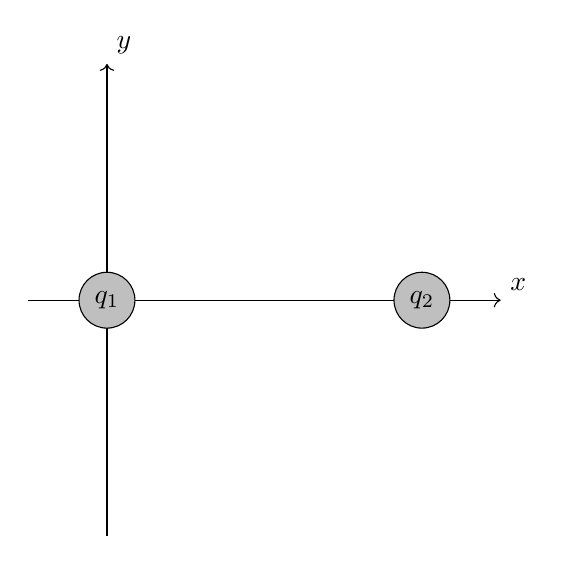
\begin{tikzpicture}
      \draw[->] (0,-3) -- (0,3) node[anchor=south west] {$y$};
      \draw[->] (-1,0) -- (5,0) node[anchor=south west] {$x$};
    
    
      \node[shape=circle,draw,fill=gray!50] at (0,0) {$q_1$};
      \node[shape=circle,draw,fill=gray!50] at (4,0) {$q_2$};

    
    \end{tikzpicture}
    
  \end{multicols}



}

\vs

\content

\vs \hrule \vs 

\content 

\vs


\end{document}